
\documentclass[a4paper, twoside]{article}
\usepackage[backend=biber,style=ieee,sorting=none]{biblatex}
\usepackage{geometry}
\geometry{a4paper,total={170mm,250mm},left=20mm, top=20mm,}
\usepackage{enumerate}
\usepackage[shortlabels]{enumitem}
\usepackage{optidef}
\usepackage[normalem]{ulem}
\useunder{\uline}{\ul}{}
\addbibresource{mybibliography.bib}
\usepackage{datetime}
\usepackage{tableof}
\usepackage{amssymb}
\usepackage{algpseudocode}
\usepackage{multirow}
\usepackage{graphicx}
\usepackage{amsmath}
\usepackage{pdfpages}

\newdateformat{monthyeardate}{%
  \monthname[\THEMONTH], \THEYEAR}
\date{\monthyeardate\today}
%%%%%%%%%%%%%%%%%%%%%%%%%%%%%%%%%%%%%%%%%%%%%%%%%%%%%%%%%%%%%%%%%%%%%%%%%%%%%%%%%%%%%
%%%%%%%%%%%%%%%%%%%%%%%%%%%   Enter Your info here    %%%%%%%%%%%%%%%%%%%%%%%%%%%%%%%

\author{Benjamin Tollison}
\def\snum{Author}
\def\coursecode{AERO423}
\def\coursetitle{Orbital Mechanics}
\def\assignname{Final Project A}

\title{Fall 23 Project}

%%%%%%%%%%%%%%%%%%%%%%%%%%%%%%%%%%%%%%%%%%%%%%%%%%%%%%%%%%%%%%%%%%%%%%%%%%%%%%%%%%%%%%



\begin{document}
\begin{titlepage}

\newcommand{\HRule}{\rule{\linewidth}{0.5mm}} % Defines a new command for the horizontal lines, change thickness here

%----------------------------------------------------------------------------------------
%	LOGO SECTION
%----------------------------------------------------------------------------------------
\centering

\includegraphics[width=8cm]{title/logo.png}\\[1cm] % Include a department/university logo - this will require the graphicx package
 
%----------------------------------------------------------------------------------------

\center % Center everything on the page

%----------------------------------------------------------------------------------------
%	HEADING SECTIONS
%----------------------------------------------------------------------------------------

\textsc{\LARGE \assignname}\\[1.5cm] %assignment name
\textsc{\Large \coursecode}\\[0.5cm] %Course code 
\textsc{\large \coursetitle}\\[0.5cm]  %Course title

%----------------------------------------------------------------------------------------
%	TITLE SECTION
%----------------------------------------------------------------------------------------
\makeatletter
\HRule \\[0.4cm]
{ \huge \bfseries \@title}\\[0.4cm] % Title of your document
\HRule \\[1.5cm]
 
%----------------------------------------------------------------------------------------
%	AUTHOR SECTION
%----------------------------------------------------------------------------------------

\begin{minipage}{0.4\textwidth}
\begin{flushleft} \large
\emph{Group Members}\\
\text{Jirina Bredberg}\\[1.2em]
\text{Ines Meyer}\\[1.2em]
\text{Kanishka Kamal}\\[1.2em]
\@author\\[1.2em] % Your name
\end{flushleft}
\end{minipage}
~
\begin{minipage}{0.4\textwidth}
\begin{flushright} \large
\emph{Tasks} \\
\text{Tables 1,2,5} \\[1.2em] 
\text{Tables 1,3,7} \\[1.2em] 
\text{Tables 3,4,6}\\[1.2em] 
\text{Author/Debugger,8} \\[1.2em] 
\end{flushright}
\end{minipage}\\[2cm]
\makeatother

%----------------------------------------------------------------------------------------
%	DATE SECTION
%----------------------------------------------------------------------------------------

{\large \today}\\[2cm] % Date, change the \today to a set date if you want to be precise

\vfill % Fill the rest of the page with whitespace

\end{titlepage}
% 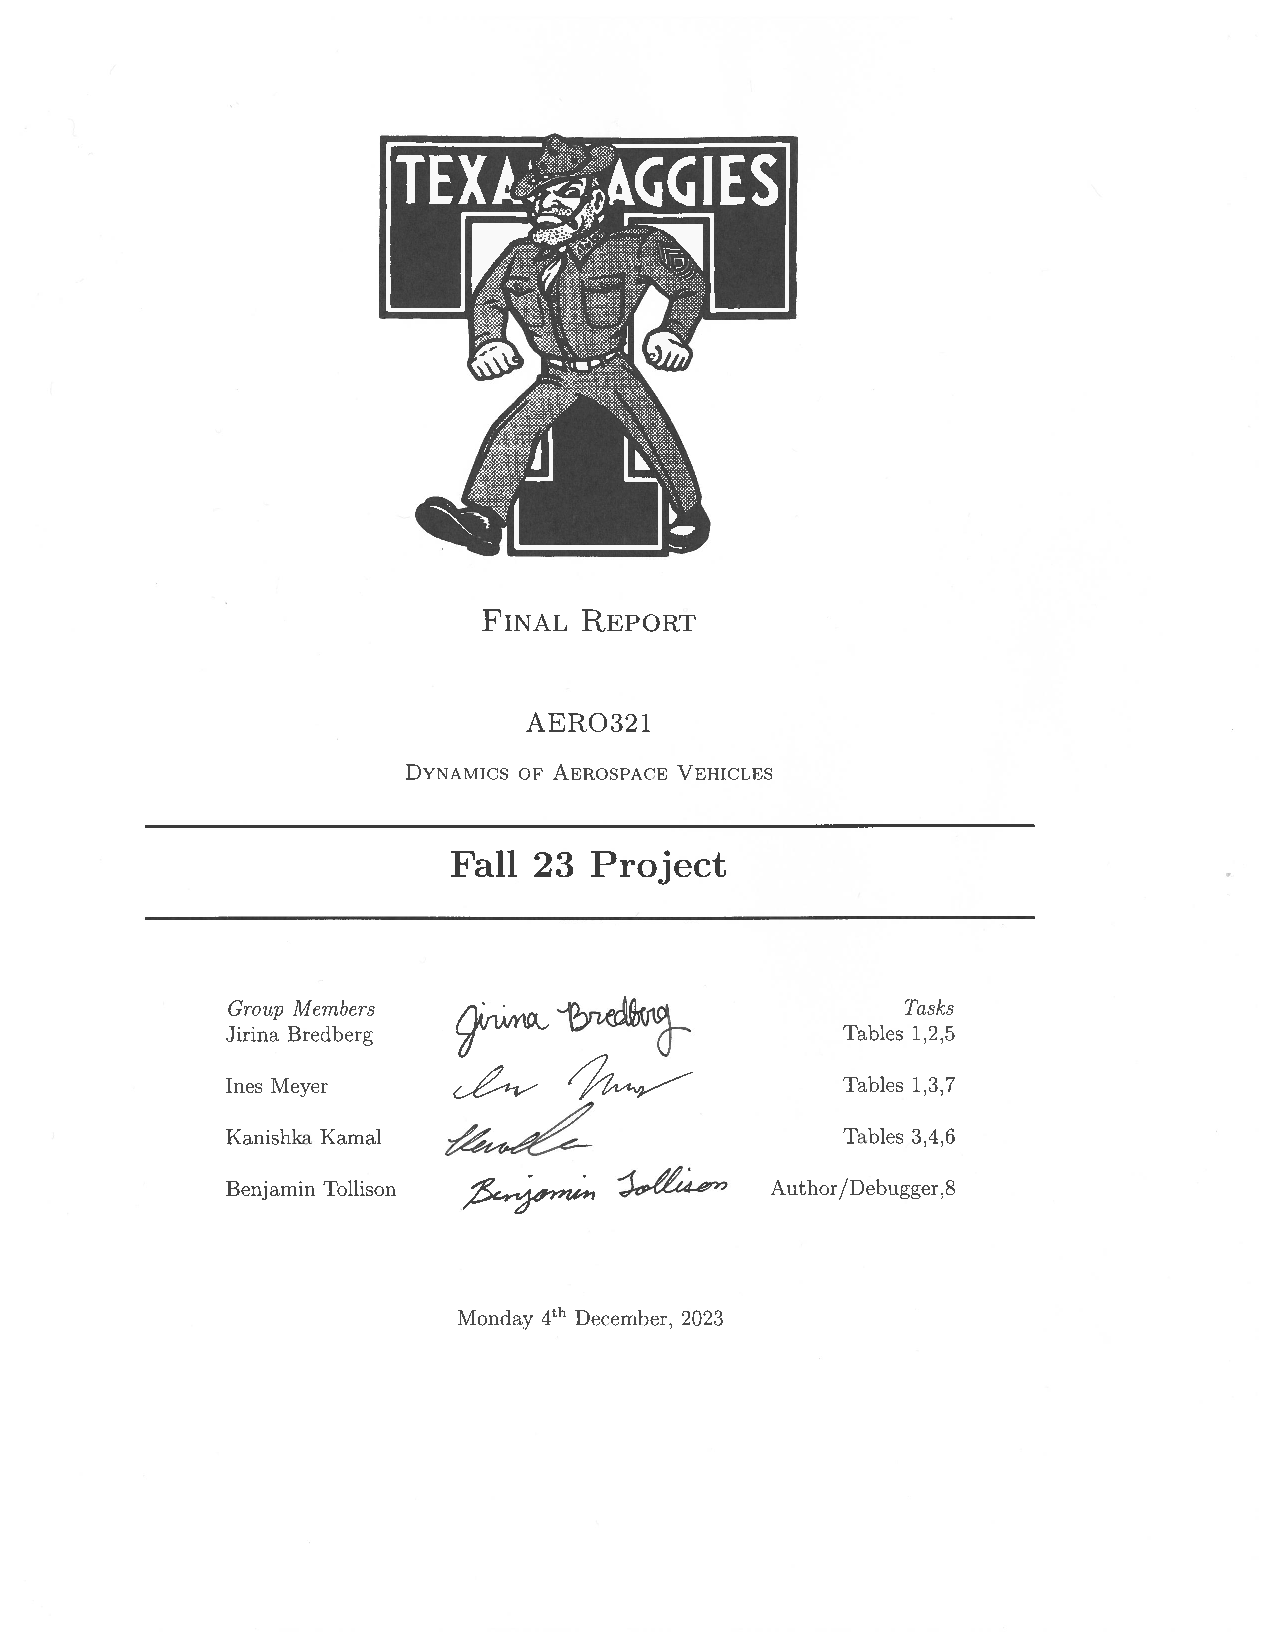
\includepdf{321ProjectTitlePage.pdf}
\tableofcontents
\newpage
\section{Project Constraints}
\begin{enumerate}
   \item \textbf{UIN:} 428004920
   \item \textbf{Orbit Altitude (\(h_{\text{alt}}\)):} 1100 km
   \item \textbf{Minimum Grazing Angle (\(\epsilon_{\min}\)):} \(12.5^{\circ}\)
   \item \textbf{Earth Radius (\(Re\)):} 6378.1365 km
   \item \textbf{Locations:}
   \begin{enumerate}
      \item Chicago, IL: \(41.8781^\circ \text{N}, 87.6298^\circ \text{W}\)
      \item Melbourne, Australia: \(37.8136^\circ \text{S}, 144.9631^\circ \text{E}\)
      \item Cape Town, South Africa: \(33.9249^\circ \text{S}, 18.4241^\circ \text{E}\)
      \item Mombasa, Kenya: \(4.0435^\circ \text{S}, 39.6682^\circ \text{E}\)
   \end{enumerate}
\end{enumerate}

\section{Initial Approximation}
Starting from the minimum number of satellites equation:
\[N_{\text{sat,min}} = \frac{2\alpha}{1-\cos{\Lambda_{\min}}}\]
and using the northernmost and southernmost latitudes to find the proportion of the Earth coverage that we want.
\begin{center}
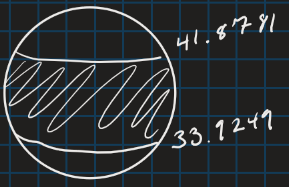
\includegraphics{alpha-coverage.png}    
\end{center}
To create the \(0<\alpha<1\):
\[\alpha = \frac{41.8781 + 33.9248}{180} = 0.42113\]

\subsection{Finding \(\Lambda_{\min}\)}
Starting from the definition of the Earth angle or half swath angle:
\[\Lambda = 90 - \epsilon - \eta\]
And \(\eta\) can be found with
\[\sin\eta = \frac{Re}{Re + h}\cos\epsilon\]
\[\eta = \arcsin{\left(\frac{Re}{Re+h}\cos\epsilon\right)}\]
\[\eta = 56.376^{\circ}\]
Which then going back to the \(\Lambda\) equation
\begin{center}
   \[\therefore \Lambda = 21.124^{\circ}\] 
\end{center}
With all of the unknowns solved in the \(N_{\text{sat,min}}\) equation produces
\[N_{\text{sat,min}} = 12.534 \rightarrow 13\]
\subsection{Finding Number of planes}
\[N_P = \frac{180}{2\Lambda + \omega_E \mathcal{TP}}\]
Where \(\mathcal{TP} = \sqrt{\frac{a^3}{\mu}}\), \(\omega_E = -0.2507\), and \(a = Re + h\)
\[N_P \rightarrow 12\]
Please be aware that the aforementioned approximation for the minimum number of satellites 
is specifically calculated under the condition of achieving 100\% coverage without any intervals 
of downtime or gaps.
\section{STK}
With the newest update of STK 12 (12.7) the Pro version got the walker function removed and moved to Premium/Enterprise, which was the tool that I used previously.
The work around that I found using the newer satellite collection tool based off of a parent satellite and sensor, 
a constellation of places, and a chain grouping. However, to check the gap times between the satellite and locations can be found
by going to the constellation>properties>constraints>logical restriction and changing both access positions to 'None Of'. This now only
checks when there are now sensors availible and then will show that time value in the report.
\\
\\
I also converted the gap times to seconds because that is what STK outputs to
\[900<Gap_{avg}<2700,Gap_{\max} = 6000\]
Here is a table of my guesses I used to narrow down to the final result of 6 satellites.
\begin{center}   
\begin{tabular}{cccccc}
  Number of Planes & Sat per plane & \(Gap_{avg}\) [s] & \(Gap_{\max}\) [s] & Total Satellites\\
  12 & 18 & 0 & 0 & 216\\
  12 & 4 & 297.572 & 518.891 & 48\\
  4 & 4 & 1122.903 & 1636.637 & 16\\
  3 & 4 & 1131.256 & 5633.492 & 12\\
  2 & 3 & 2363.21 & 16205.976 & 6\\
  6 & 1 & 2352.093 & 4648.74 & 6 \\
  5 & 1 & 2866.598 & 7241.465 & 5 \\
  3 & 2 & 2345.584 & 10589.942 & 6
\end{tabular}
\end{center}
The peculiar thing that happens with the circular orbit, and an inclination of 37 degrees, is the the locations, almost naturally, fall in
line with the orbit path such that to have the gap times is half of the predicted 100\% coverage of the 
\(\alpha\). Below is the parent satellite that the constellation is based off of.
\begin{center}
   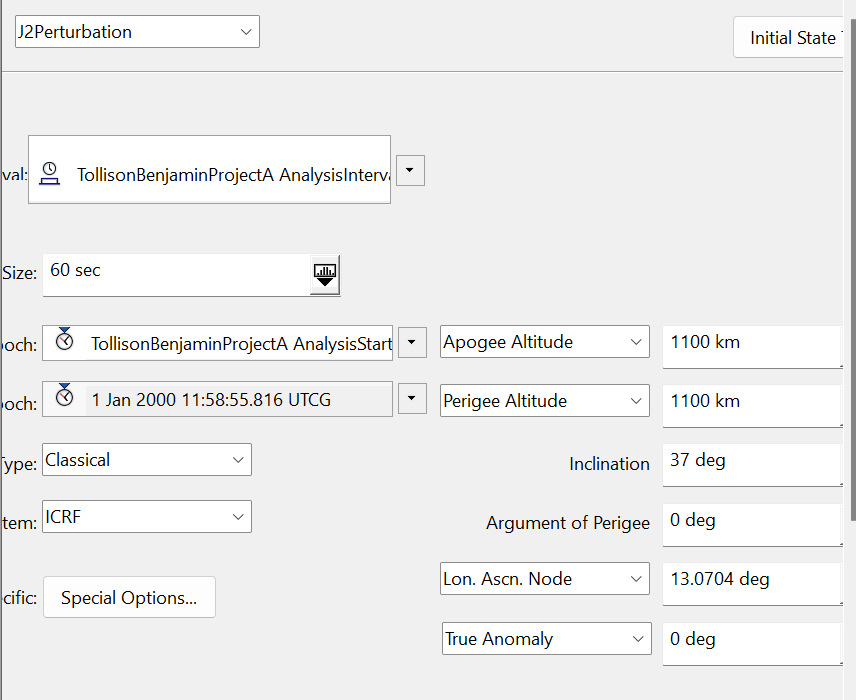
\includegraphics{parent-sat.png}
\end{center}
This is an example of how the Satellite's ground path naturally align for easier coverage.
\begin{center}
  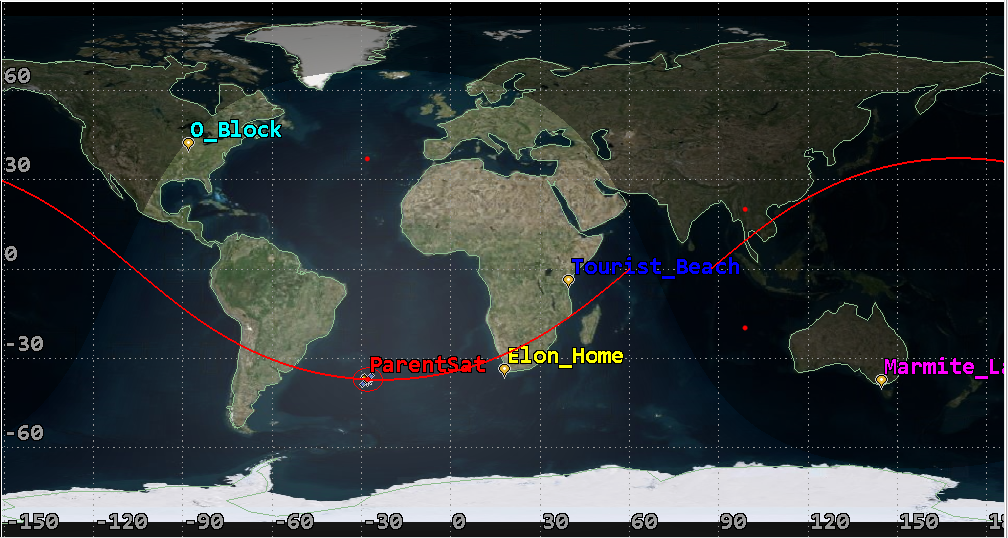
\includegraphics[width=\linewidth]{orbit-path-a.png} 
\end{center}
\pagebreak
Below is another path that covers all the orbits in 3 revolutions around Earth because of the J2 drift
\begin{center}
  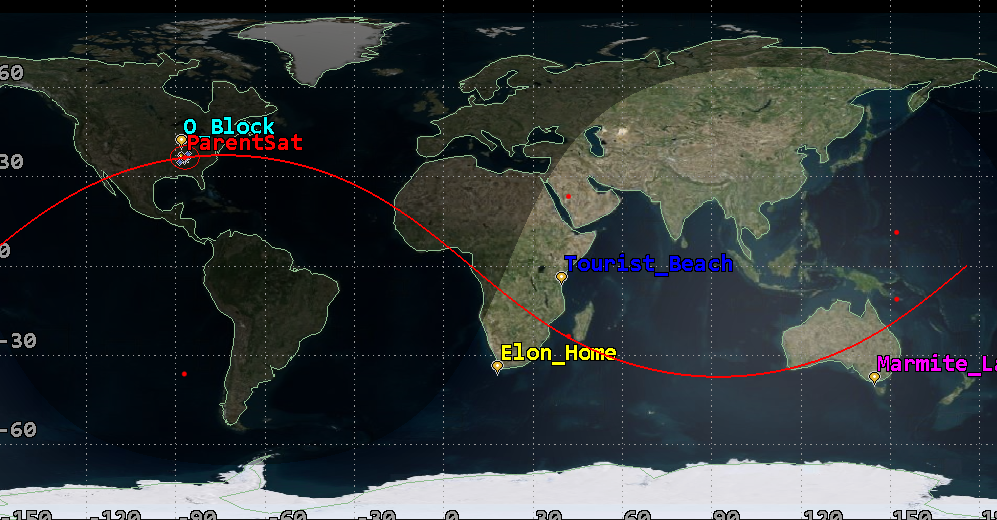
\includegraphics[width=\linewidth]{orbit-path-b.png} 
\end{center}
\subsection{Final Proposed Design}
The ultimate configuration for the satellite constellation involves six planes, 
each accommodating a single satellite. These planes are strategically positioned 
with a 60-degree offset from one another. As a result of this arrangement, 
the average gap time is anticipated to approach 39 minutes, while the maximum gap 
time is estimated to be approximately 77.5 minutes. Despite the fact that the proposed 
design aligns with the upper bounds of the specified constraints, it remains within the 
defined limitations.

\section{Code}
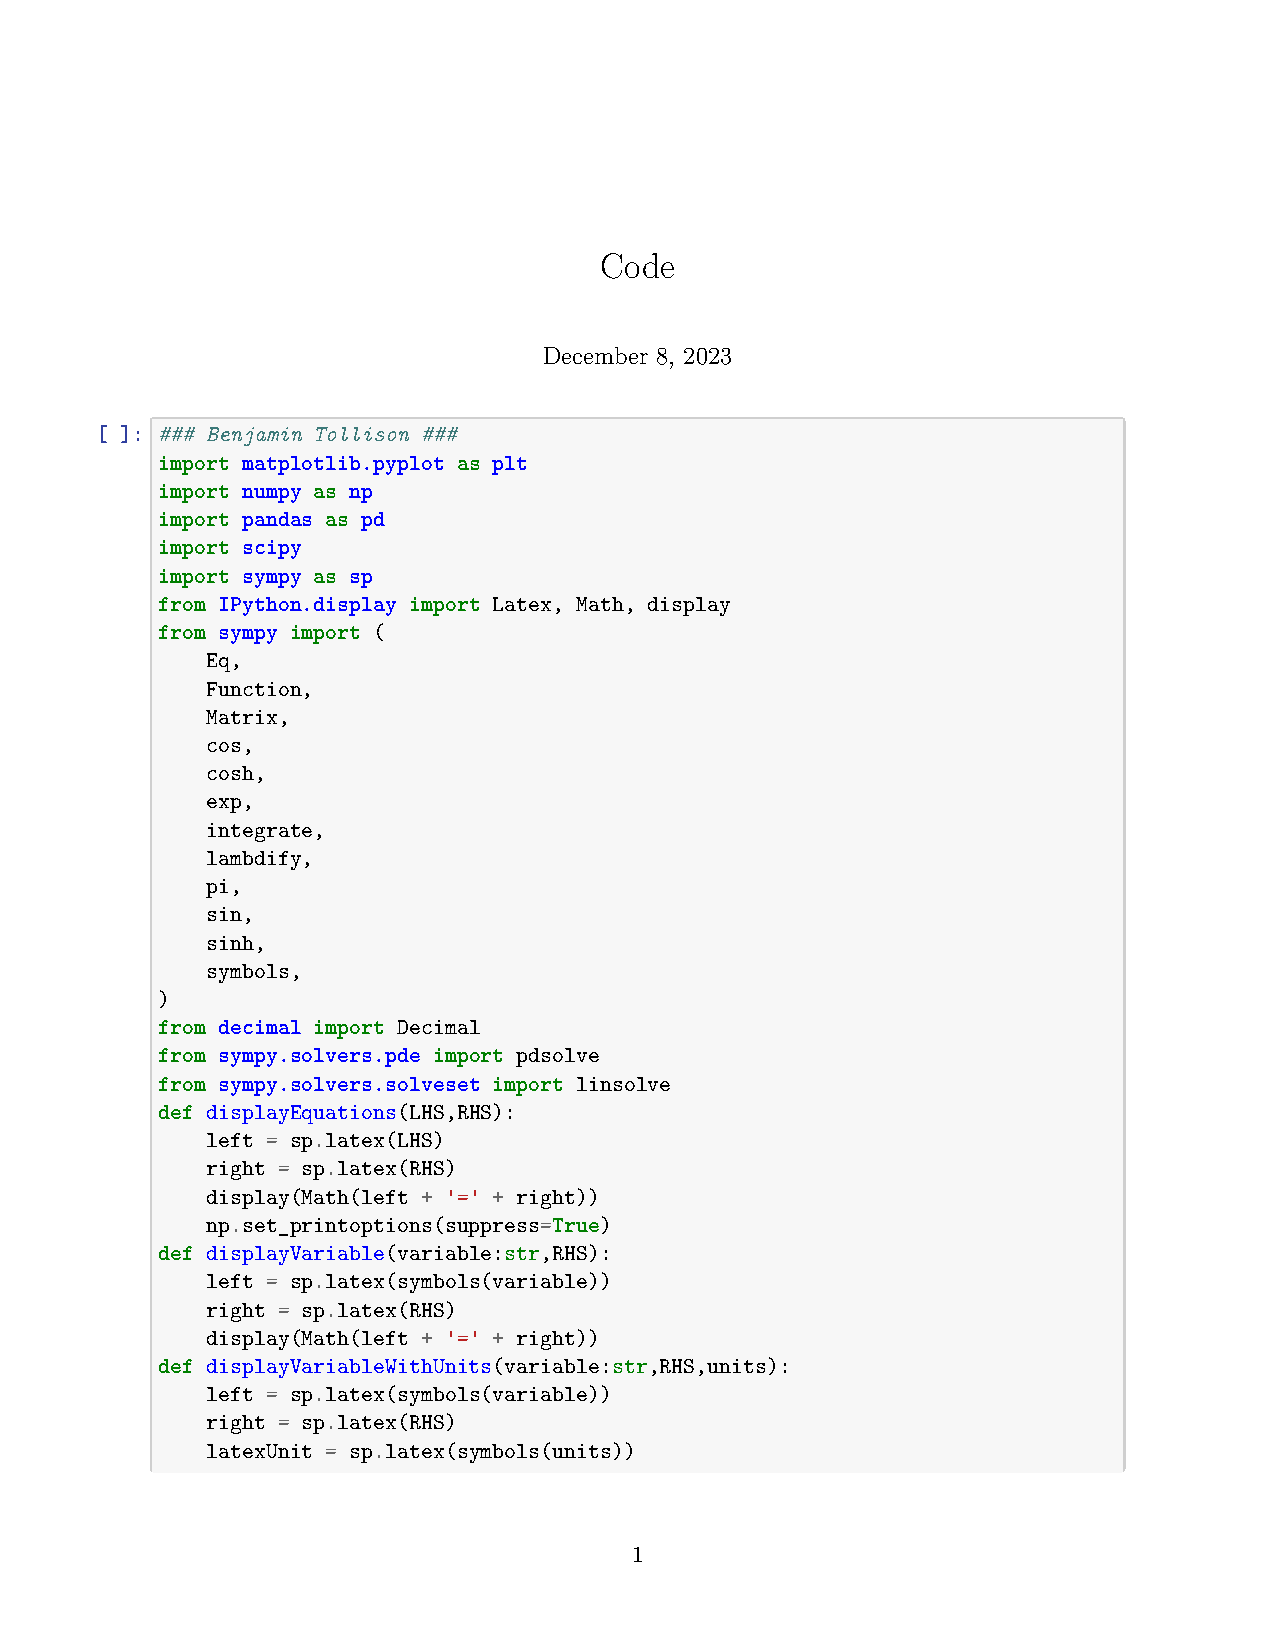
\includepdf[pages=-]{Code.pdf}



\end{document}